\documentclass[a4paper]{article}

\usepackage[english]{babel}
\usepackage[utf8]{inputenc}
\usepackage{apacite}
\usepackage{graphicx}
\usepackage{tikz}
\usepackage{xcolor}
\usepackage[colorinlistoftodos]{todonotes}

\makeatletter
\def\BState{\State\hskip-\ALG@thistlm}
\makeatother

\title{Gameplay Design \\ Assignment 2 }

\author{
  Bowald, Johan\\
  \texttt{bowaldj@student.chalmers.se}
  \and
  Odbjer, Sebastian\\
  \texttt{sebastian.odbjer@gmail.com}
}

\date{\today}

\tikzset{
    vertex/.style = {
        circle,
        fill            = black,
        outer sep = 2pt,
        inner sep = 1pt,
    }
}

\begin{document}
\maketitle
\newpage

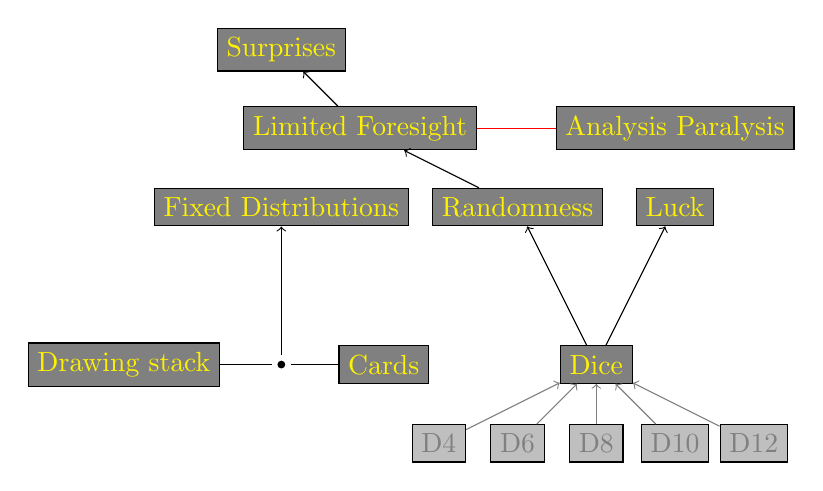
\begin{tikzpicture}
  % Dialectics
  \node[draw,fill=gray,text=yellow] (DrawingStack) at (-1,0) {Drawing stack};
  \node[draw,fill=gray,text=yellow] (Cards) at (2.3,0) {Cards};
  \node[draw,fill=gray,text=yellow] (FixedDistributions) at (1,2) {Fixed Distributions};
  
  \draw node[vertex] (Joint) at (1,0) {};
  
  \draw[-,draw=black] (DrawingStack) to (Joint);
  \draw[-,draw=black] (Cards) to (Joint);
  \draw[->,draw=black] (Joint) to (FixedDistributions);
  
  
  
  % Dice
  \node[draw,fill=gray,text=yellow] (Dice) at (5,0) {Dice};

  \node[draw,fill=gray!50,text=gray] (D4) at (3,-1) {D4};
  \node[draw,fill=gray!50,text=gray] (D6) at (4,-1) {D6};
  \node[draw,fill=gray!50,text=gray] (D8) at (5,-1) {D8};
  \node[draw,fill=gray!50,text=gray] (D10) at (6,-1) {D10};
  \node[draw,fill=gray!50,text=gray] (D12) at (7,-1) {D12};
  \draw[->,draw=gray] (D4) to (Dice);
  \draw[->,draw=gray] (D6) to (Dice);
  \draw[->,draw=gray] (D8) to (Dice);
  \draw[->,draw=gray] (D10) to (Dice);
  \draw[->,draw=gray] (D12) to (Dice);
  
  
  % Dice tier 2
  \node[draw,fill=gray,text=yellow] (Randomness) at (4,2) {Randomness};
  \node[draw,fill=gray,text=yellow] (Luck) at (6,2) {Luck};
  
  \draw[->,draw=black] (Dice) to (Randomness);
  \draw[->,draw=black] (Dice) to (Luck);
    
  % Dice tier 3
  \node[draw,fill=gray,text=yellow] (LimitedForesight) at (2,3) {Limited Foresight};
  \node[draw,fill=gray,text=yellow] (AnalysisParalysis) at (6,3) {Analysis Paralysis};
  
  \draw[->,draw=black] (Randomness) to (LimitedForesight);
  \draw[-,draw=red] (LimitedForesight) to (AnalysisParalysis);

  \node[draw,fill=gray,text=yellow] (Surprises) at (1,4) {Surprises};
  \draw[->,draw=black] (LimitedForesight) to (Surprises);
  
\end{tikzpicture}

\newpage
\bibliographystyle{apacite}
\bibliography{bib}

\end{document} 

